\documentclass[12pt]{article}
\usepackage[margin=2.5cm]{geometry}
\usepackage{enumerate}
\usepackage{amsfonts}
\usepackage{amsmath}
\usepackage{fancyhdr}
\usepackage{amsmath}
\usepackage{amssymb}
\usepackage{amsthm}
\usepackage{mdframed}
\usepackage{graphicx}
\usepackage{subcaption}
\usepackage{adjustbox}
\usepackage{listings}
\usepackage{xcolor}
\usepackage{booktabs}
\usepackage[utf]{kotex}
\usepackage{hyperref}

\definecolor{codegreen}{rgb}{0,0.6,0}
\definecolor{codegray}{rgb}{0.5,0.5,0.5}
\definecolor{codepurple}{rgb}{0.58,0,0.82}
\definecolor{backcolour}{rgb}{0.95,0.95,0.92}

\lstdefinestyle{mystyle}{
    backgroundcolor=\color{backcolour},
    commentstyle=\color{codegreen},
    keywordstyle=\color{magenta},
    numberstyle=\tiny\color{codegray},
    stringstyle=\color{codepurple},
    basicstyle=\ttfamily\footnotesize,
    breakatwhitespace=false,
    breaklines=true,
    captionpos=b,
    keepspaces=true,
    numbers=left,
    numbersep=5pt,
    showspaces=false,
    showstringspaces=false,
    showtabs=false,
    tabsize=1
}

\lstset{style=mystyle}

\pagestyle{fancy}
\renewcommand{\headrulewidth}{0.4pt}
\lhead{Team Treehouse}
\rhead{Local Development Environment Part 2 Notes}

\begin{document}
\title{Local Development Environment Part 2 Notes}
\author{Team Treehouse}
\maketitle

\section{Introducing IDEs}

\bigskip

\begin{itemize}
    \item \textbf{Installing IntelliJ IDEA:} Can be done \href{http://treehouse.github.io/installation-guides/mac/intellij-idea-mac.html}{here}
\end{itemize}

\bigskip

\section{Creating Your First Project}

\bigskip

\begin{itemize}

    \item Creating Project
    \begin{enumerate}[1.]
        \item Choose Project SDK


        \begin{center}
        
\includegraphics[width=\linewidth]{images/part_2_notes_1.png}
        \end{center}

        \bigskip

        \underline{\textbf{Notes:}}

        \bigskip

        \begin{itemize}
            \item The part about `Additional Libraries and Framework' can be ommitted
        \end{itemize}

        \begin{center}
        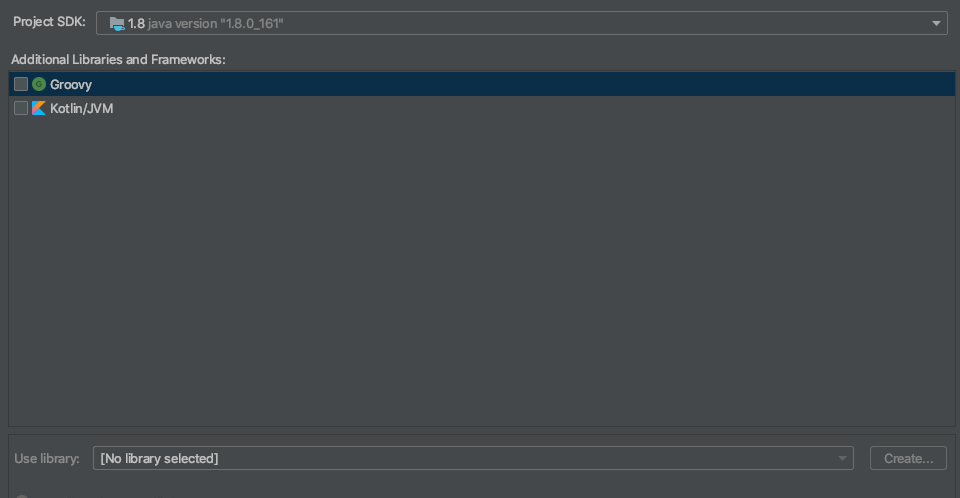
\includegraphics[width=\linewidth]{images/part_2_notes_2.png}
        \end{center}

        \item Choose template `Command Line App'

        \begin{center}
        
\includegraphics[width=\linewidth]{images/part_2_notes_3.png}
        \end{center}

        \item Set project name `Systemizer'

        \item Generate Project
    \end{enumerate}

    \item Running project

    \begin{enumerate}[1.]
        \item By pressing \textit{Run `Main'} under \textit{RUN} menu

        \begin{center}
        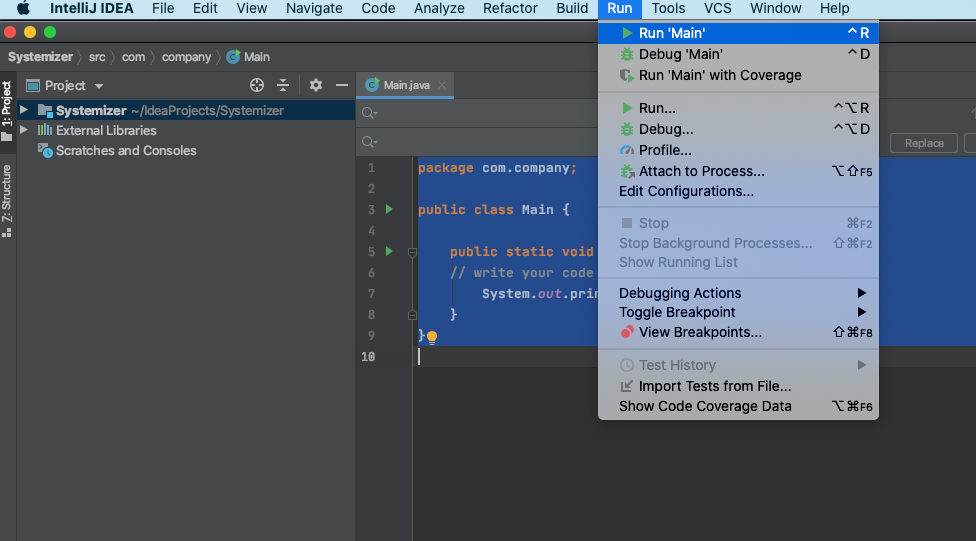
\includegraphics[width=\linewidth]{images/part_2_notes_4.png}
        \end{center}
    \end{enumerate}

\end{itemize}
\end{document}